%% BioMed_Central_Tex_Template_v1.06
%%                                      %
%  bmc_article.tex            ver: 1.06 %
%                                       %

%%IMPORTANT: do not delete the first line of this template
%%It must be present to enable the BMC Submission system to
%%recognise this template!!

%%%%%%%%%%%%%%%%%%%%%%%%%%%%%%%%%%%%%%%%%
%%                                     %%
%%  LaTeX template for BioMed Central  %%
%%     journal article submissions     %%
%%                                     %%
%%          <8 June 2012>              %%
%%                                     %%
%%                                     %%
%%%%%%%%%%%%%%%%%%%%%%%%%%%%%%%%%%%%%%%%%


%%%%%%%%%%%%%%%%%%%%%%%%%%%%%%%%%%%%%%%%%%%%%%%%%%%%%%%%%%%%%%%%%%%%%
%%                                                                 %%
%% For instructions on how to fill out this Tex template           %%
%% document please refer to Readme.html and the instructions for   %%
%% authors page on the biomed central website                      %%
%% http://www.biomedcentral.com/info/authors/                      %%
%%                                                                 %%
%% Please do not use \input{...} to include other tex files.       %%
%% Submit your LaTeX manuscript as one .tex document.              %%
%%                                                                 %%
%% All additional figures and files should be attached             %%
%% separately and not embedded in the \TeX\ document itself.       %%
%%                                                                 %%
%% BioMed Central currently use the MikTex distribution of         %%
%% TeX for Windows) of TeX and LaTeX.  This is available from      %%
%% http://www.miktex.org                                           %%
%%                                                                 %%
%%%%%%%%%%%%%%%%%%%%%%%%%%%%%%%%%%%%%%%%%%%%%%%%%%%%%%%%%%%%%%%%%%%%%

%%% additional documentclass options:
%  [doublespacing]
%  [linenumbers]   - put the line numbers on margins

%%% loading packages, author definitions

\documentclass[twocolumn]{bmcart}% uncomment this for twocolumn layout and comment line below
%\documentclass{bmcart}

%%% Load packages
%\usepackage{amsthm,amsmath}
\RequirePackage{natbib}
%\RequirePackage[authoryear]{natbib}% uncomment this for author-year bibliography
%\RequirePackage{hyperref}
\usepackage[utf8]{inputenc} %unicode support
%\usepackage[applemac]{inputenc} %applemac support if unicode package fails
%\usepackage[latin1]{inputenc} %UNIX support if unicode package fails


% Load bibliography package dany
\usepackage{natbib}
\usepackage{graphicx}
\graphicspath{ {images/} }
\usepackage{hyperref}

%%%%%%%%%%%%%%%%%%%%%%%%%%%%%%%%%%%%%%%%%%%%%%%%%
%%                                             %%
%%  If you wish to display your graphics for   %%
%%  your own use using includegraphic or       %%
%%  includegraphics, then comment out the      %%
%%  following two lines of code.               %%
%%  NB: These line *must* be included when     %%
%%  submitting to BMC.                         %%
%%  All figure files must be submitted as      %%
%%  separate graphics through the BMC          %%
%%  submission process, not included in the    %%
%%  submitted article.                         %%
%%                                             %%
%%%%%%%%%%%%%%%%%%%%%%%%%%%%%%%%%%%%%%%%%%%%%%%%%


%\def\includegraphic{}
%\def\includegraphics{}



%%% Put your definitions there:
\startlocaldefs
\endlocaldefs


%%% Begin ...
\begin{document}

%%% Start of article front matter
\begin{frontmatter}

\begin{fmbox}
\dochead{Research}

%%%%%%%%%%%%%%%%%%%%%%%%%%%%%%%%%%%%%%%%%%%%%%
%%                                          %%
%% Enter the title of your article here     %%
%%                                          %%
%%%%%%%%%%%%%%%%%%%%%%%%%%%%%%%%%%%%%%%%%%%%%%

\title{Evaluación diagnóstica diabética con aprendizaje automático }

%%%%%%%%%%%%%%%%%%%%%%%%%%%%%%%%%%%%%%%%%%%%%%
%%                                          %%
%% Enter the authors here                   %%
%%                                          %%
%% Specify information, if available,       %%
%% in the form:                             %%
%%   <key>={<id1>,<id2>}                    %%
%%   <key>=                                 %%
%% Comment or delete the keys which are     %%
%% not used. Repeat \author command as much %%
%% as required.                             %%
%%                                          %%
%%%%%%%%%%%%%%%%%%%%%%%%%%%%%%%%%%%%%%%%%%%%%%

\author[
   addressref={aff1},                   % id's of addresses, e.g. {aff1,aff2}
   corref={aff1},                       % id of corresponding address, if any
   %noteref={n1},                        % id's of article notes, if any
   email={joel.rodarter@uanl.edu.mx}   % email address
]{\inits{JE}\fnm{Joel Alejandro} \snm{Rodarte Rivera}}


%%%%%%%%%%%%%%%%%%%%%%%%%%%%%%%%%%%%%%%%%%%%%%
%%                                          %%
%% Enter the authors' addresses here        %%
%%                                          %%
%% Repeat \address commands as much as      %%
%% required.                                %%
%%                                          %%
%%%%%%%%%%%%%%%%%%%%%%%%%%%%%%%%%%%%%%%%%%%%%%

\address[id=aff1]{%                           % unique id
  \orgname{Facultad de Ciencias Fisicomatemática,UANL}, % university, etc
 % \street{Waterloo Road},                     %
  %\postcode{}                                % post or zip code
  \city{Monterrey, Nuevo Léon},                              % city
  \cny{México}                                    % country
}

%%%%%%%%%%%%%%%%%%%%%%%%%%%%%%%%%%%%%%%%%%%%%%
%%                                          %%
%% Enter short notes here                   %%
%%                                          %%
%% Short notes will be after addresses      %%
%% on first page.                           %%
%%                                          %%
%%%%%%%%%%%%%%%%%%%%%%%%%%%%%%%%%%%%%%%%%%%%%%

%\begin{artnotes}
%\note{Sample of title note}     % note to the article
%\note[id=n1]{Equal contributor} % note, connected to author
%\end{artnotes}

\end{fmbox}% comment this for two column layout

%%%%%%%%%%%%%%%%%%%%%%%%%%%%%%%%%%%%%%%%%%%%%%
%%                                          %%
%% The Abstract begins here                 %%
%%                                          %%
%% Please refer to the Instructions for     %%
%% authors on http://www.biomedcentral.com  %%
%% and include the section headings         %%
%% accordingly for your article type.       %%
%%                                          %%
%%%%%%%%%%%%%%%%%%%%%%%%%%%%%%%%%%%%%%%%%%%%%%

\begin{abstractbox}

\begin{abstract} % abstract

El presente escrito tiene como objetivo el clasificar pacientes que dado los resultados de presencia o ausencia de 142 síntomas, se pueda determinar si es diagnosticado como diabético. Se analiza un conjunto de datos con 4,920 entradas de pacientes y 42 posibles resultados de enfermedades.  

\textbf{Métodos:} Para poder cumplir con el objetivo se utilizaron algoritmos no supervisados, supervisados, de clasifiación así como selección de características para determinar cuáles variables son las más relevantes para la clasifiación. Este documente incluye información de los algoritmos de regresión logística, árboles de desición, K medias, selección de carácteristicas por correlación y por información mutua. Algúnes métricos de desempeño fuero la presición, exactutud, estadísitco F1 y curvas ROC. 

\textbf{Resultados:} Los algoritmos dejan entrever que los síntomas que son más relevantes para comprender si un paciente pudiera tener diabetes es la polyuria, el apetito incrementado y niveles irregulares de azúcar en la sangre. La ausencia de saber información de estos síntomas pudiera comprometer a los algoritmos para entender si se diagnostica diabetes. 

\textbf{Conclusiones:} Para el conjunto de datos estudiado, si es posible dictaminar con un excelente desempeño si un paciente padece diabetes o no. Los algoritmos de regresión logística, árboles de decisión y bayes ingenuos muestran excelencia al clasificar la presencia o ausencia de diabetes ya que los tres clasifican correctamente a todos los pacientes del conjunto de prueba. La información brindada por los síntomas es suficiente para hacer predicción de conclusiones médicas. 
 

\end{abstract}

%%%%%%%%%%%%%%%%%%%%%%%%%%%%%%%%%%%%%%%%%%%%%%
%%                                          %%
%% The keywords begin here                  %%
%%                                          %%
%% Put each keyword in separate \kwd{}.     %%
%%                                          %%
%%%%%%%%%%%%%%%%%%%%%%%%%%%%%%%%%%%%%%%%%%%%%%

\begin{keyword}
\kwd{Diabetes}
\kwd{Aprendizaje Automático}
\kwd{Regresión Logística}
\kwd{Árboles de desición}
\end{keyword}

% MSC classifications codes, if any
%\begin{keyword}[class=AMS]
%\kwd[Primary ]{}
%\kwd{}
%\kwd[; secondary ]{}
%\end{keyword}

\end{abstractbox}
%
%\end{fmbox}% uncomment this for twcolumn layout

\end{frontmatter}

%%%%%%%%%%%%%%%%%%%%%%%%%%%%%%%%%%%%%%%%%%%%%%
%%                                          %%
%% The Main Body begins here                %%
%%                                          %%
%% Please refer to the instructions for     %%
%% authors on:                              %%
%% http://www.biomedcentral.com/info/authors%%
%% and include the section headings         %%
%% accordingly for your article type.       %%
%%                                          %%
%% See the Results and Discussion section   %%
%% for details on how to create sub-sections%%
%%                                          %%
%% use \cite{...} to cite references        %%
%%  \cite{koon} and                         %%
%%  \cite{oreg,khar,zvai,xjon,schn,pond}    %%
%%  \nocite{smith,marg,hunn,advi,koha,mouse}%%
%%                                          %%
%%%%%%%%%%%%%%%%%%%%%%%%%%%%%%%%%%%%%%%%%%%%%%

%%%%%%%%%%%%%%%%%%%%%%%%% start of article main body
% <put your article body there>
\section*{Introducción}

Desde su acuñamiento a mediados de siglo XX el aprendizaje automático , rama de la inteligencia artificial que se centra en el desarrollo de algoritmos y modelos que permiten a las computadoras aprender y mejorar su desempeño en una tarea específica a medida que se les proporciona más datos, ha evolucionado para solucionar problemas del mundo real en diferentes áreas. La medicina es una de las que se ha visto ampliamente beneficiada para complementar el esfuerzo de los  trabajadores de la salud. El aprendizaje automático puede ser utilizado en la medicina para explorar datos, imágenes o sonidos para así encontrar patrones difíciles de identificar. Algunos ejemplos son el análisis de imágenes radiográficas  para detectar tumores o evaluar la presencia o ausencia de una enfermedad dado unos síntomas, para así tomar decisiones más acertadas y atacar la enfermedad con rapidez o evitar cometer un error clínico. 

Justamente este es el objetivo del escrito, el cual busca determinar si un paciente, dado ciertos síntomas, es diagnosticado con diabetes. El alcance de este texto se limita a determinar si existe o no diabetes, ya que por el momento determinar si es diabetes tipo I o II no se realizará. El conjunto de datos cuenta con 4,920 pacientes para los cuales, para cada uno de ellos se tiene documentado los síntomas que presentó y el dictamen de la enfermedad que se le diagnosticó. En total, cada paciente cuenta con 132 posibles síntomas los cuáles pueden derivar en 42 enfermedades. Para el presente, los esfuerzos están dedicados a predecir diabetes pero la metodología y base de datos puede ser utilizada para cada una de las enfermedades. El conjunto de datos cuenta únicamente con información binaria, es decir ceros y unos siendo que cuando algo sea verdad es decir, que existe un síntoma o enfermedad se le coloca un uno. Todas las variables están en inglés; como comentario prognosis es una manera de llamar a una enfermedad. El grupo de datos fue encontrado en la base de datos pública de fuente abierta en Kaggle \cite{Kaggle}. Se investigó pero no se indica su procedencia o autoría por lo que los resultados de este escrito deben ser tomados como un ejercicio académico. 

Otro comentario importante por el cuál esta publicación debe ser tomada sólo como un ejercicio académico es que muy avanzada el desarrollo del mismo, y dado que los métricos de desempeño de los algoritmos eran perfectos, se comenzó a sospechar que había riesgo de sobreajuste dado que algo en el conjunto de datos estaba fuera de lugar. Investigando en los foros de la base de datos se encontró que efectivamente existía algo que podía estar generando dichos resultados. De los 4,920 registros solo se cuenta con 304 registro únicos. Esto lo que genera es que los datos sean muy homogéneos y la dispersión de los mismos no sea suficiente para generar buenos modelos de aprendizaje automático para nuevos datos. Esto también se ve reflejado en las siguientes observaciones en donde pareciera ser que todos los síntomas tienen frecuencias de aparición similares.  A continuación un pequeño análisis exploratorio de los datos para entender qué es lo que contiene. 

De entre los 4,920 registros, la siguiente tabla de frecuencias muestra los diez síntomas más comunes. La intención de tener en la mira a estos síntomas es que son los que menos información podrían aportar a la predicción de diabetes o en general de cualquier enfermedad dado que son tan comunes es decir, que están presentes en múltiples enfermedades que incluirlos en los algoritmos podrían llevar a tomar decisión incorrectas por confusión de síntomas. Los 10 síntomas más común de mayor a menor fueron fatiga, vómito, fiebre alta, pérdida de apetito, náusea, dolor de cabeza, dolor abdominal, piel amarillenta, ojos amarillentos y escalofríos. 

\begin{figure}[h!]
  \caption{\csentence{}
      Frecuencias de síntomas más comunes entre los 4920 pacientes.}
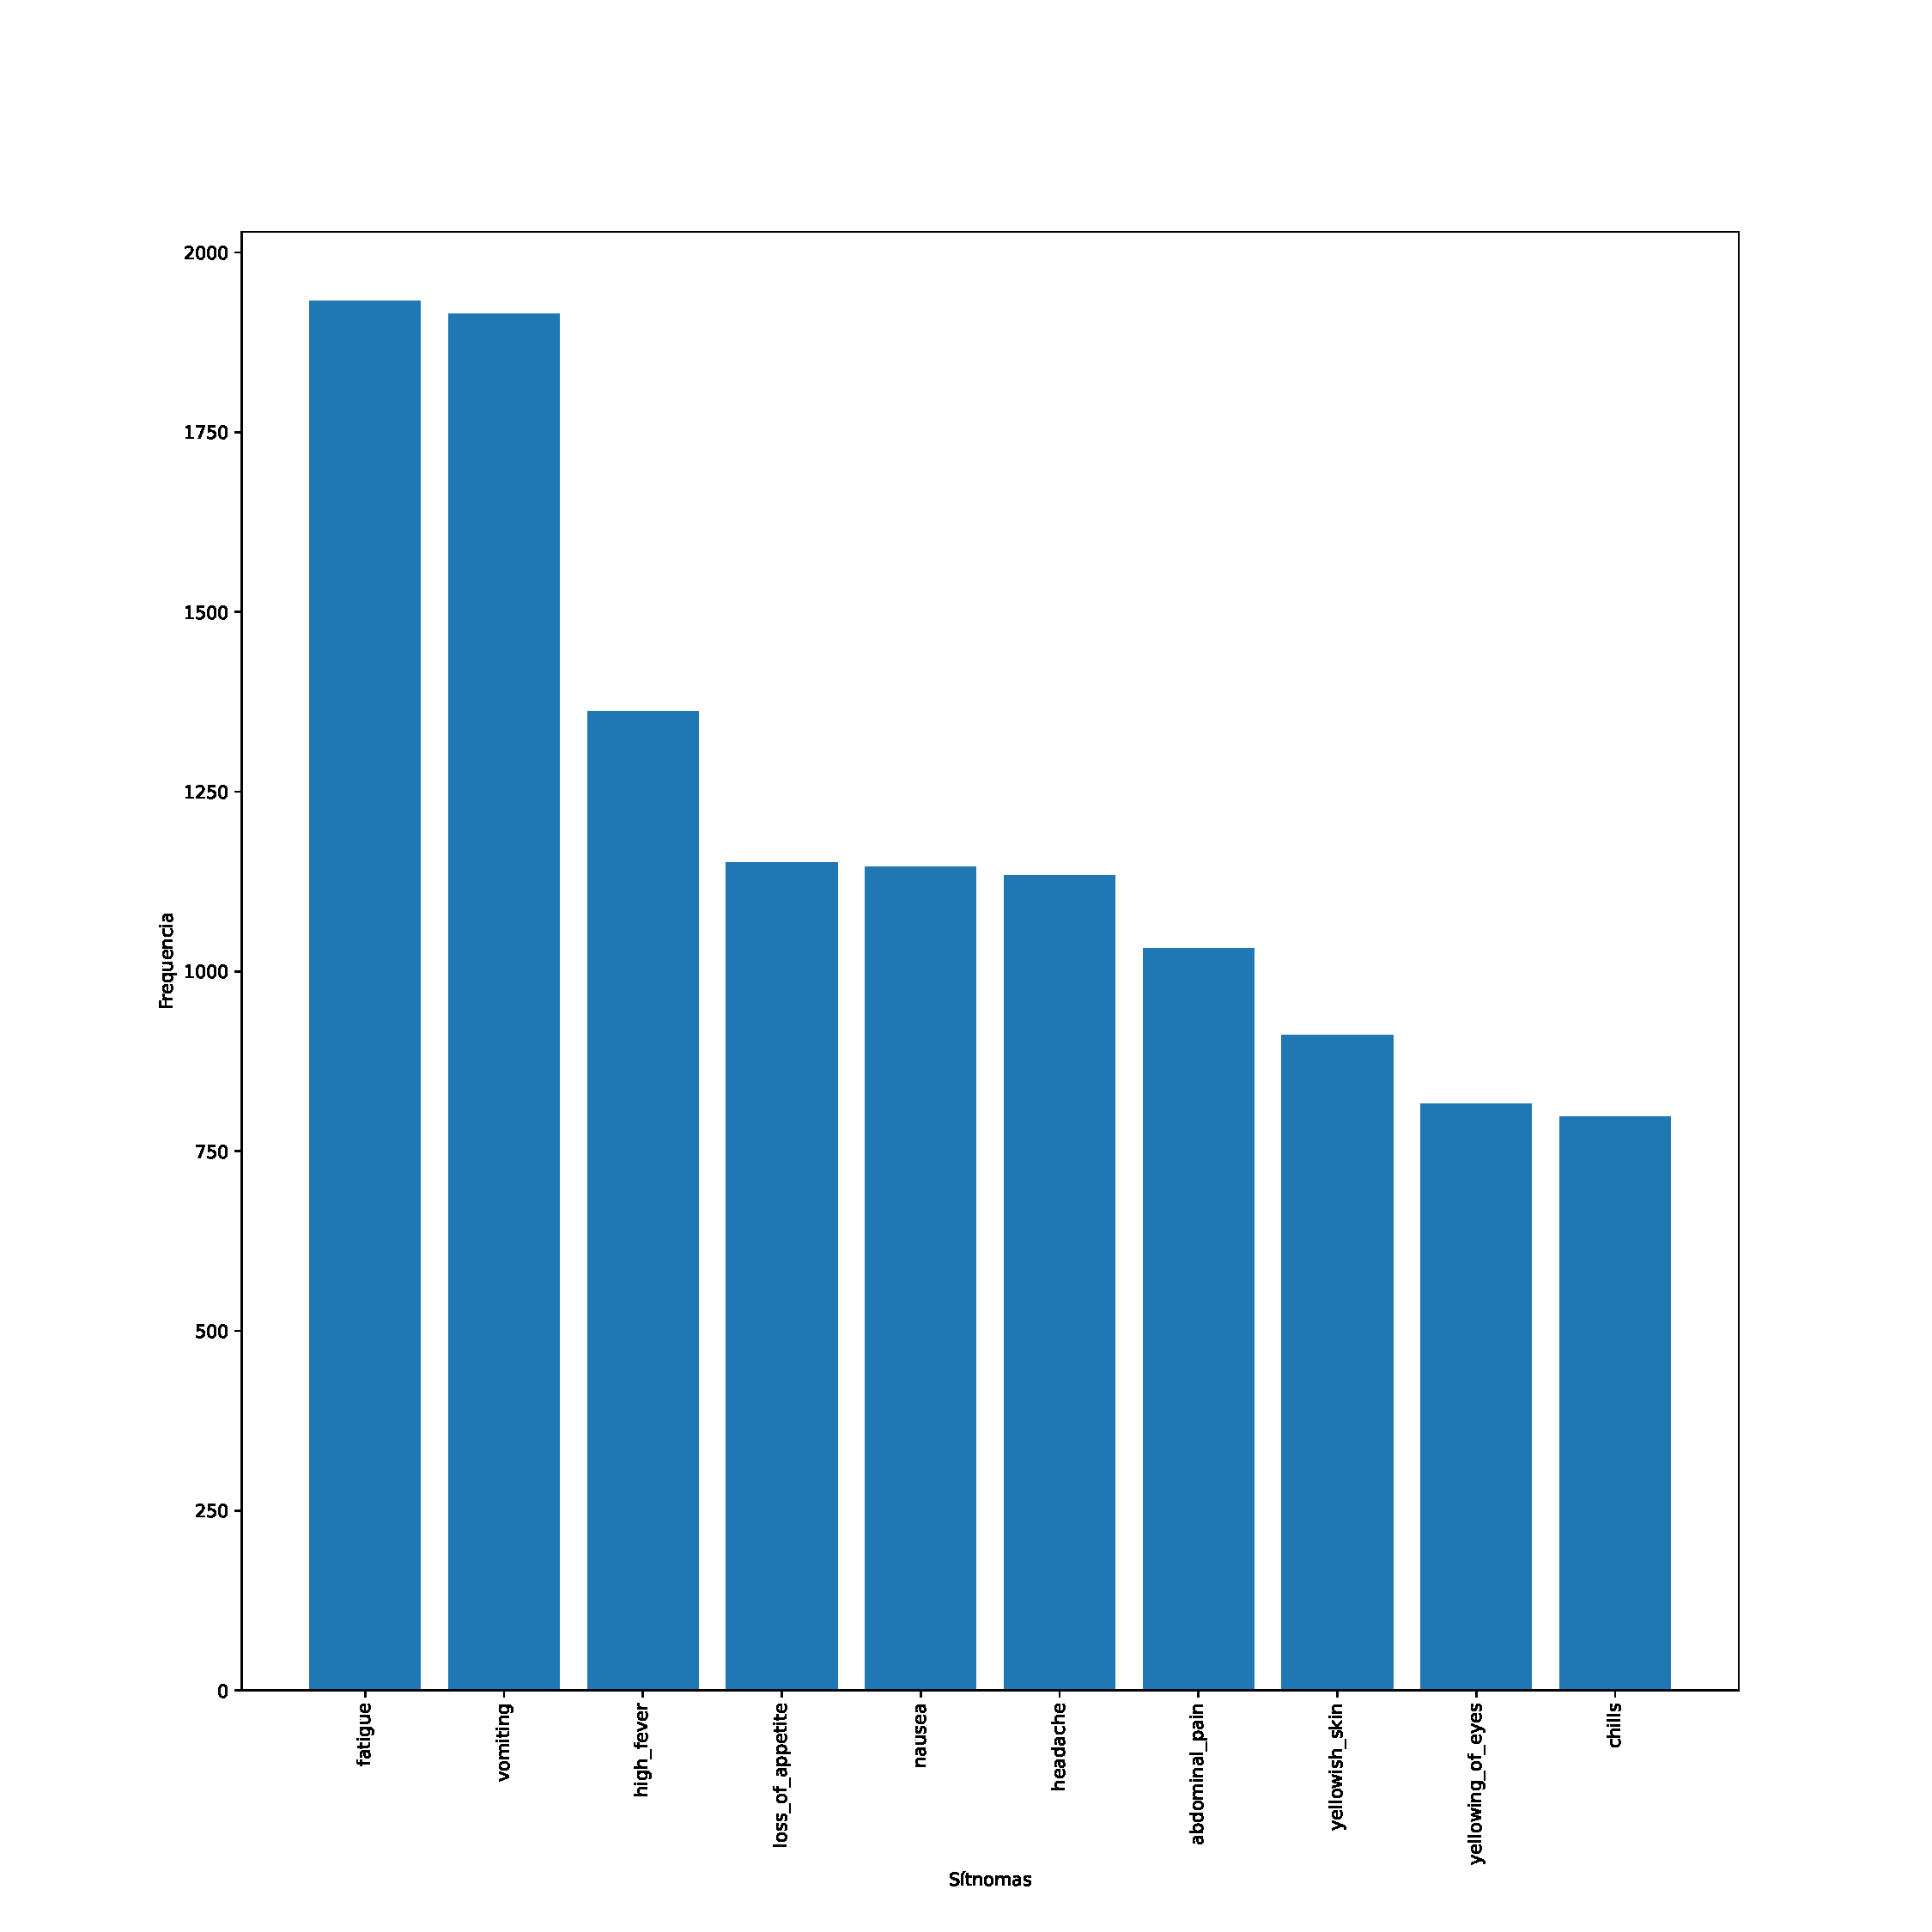
\includegraphics[scale=0.20]{images/FrecuenciaSintomas.pdf}  
      \end{figure}

Ahora que se sabe cuales son los síntomas más comunes considerando todas las enfermedades, también es importante entender cuáles son los más comunes y la frecuencia del mismo para los pacientes con diabetes. Se sabe que el conjunto de datos de entrenamiento cuenta con 120 pacientes diabéticos. A continuación los diez síntomas más comunes. Son justamente estos síntomas a los que hay que prestar atención cuando se quiere predecir diabetes. 
$$
\begin{array}{ll}
\text { increased appetite } & 120 \\
\text { polyuria } & 120 \\
\text { weight loss } & 114 \\
\text { irregular sugar_level } & 114 \\
\text { blurred and distorted vision } & 114 \\
\text { fatigue } & 114 \\
\text { lethargy } & 114 \\
\text { restlessness } & 114 \\
\text { excessive hunger } & 114 \\
\text { obesity } & 114
\end{array}
$$

Por último es importante entender en qué proporción, por cada variable de síntomas de diabetes, se encuentra también en otra enfermedad. La siguiente tabla tiene como objetivo explicar cuantas veces se presentan los síntomas en el conjunto completo y cuantas veces se presenta considerando solo los pacientes con diabetes. Si la proporción es 1, significa que únicamente los pacientes con diabetes son los que cuentan con dicho síntoma. A medida que baja la proporción significa que el síntoma a pesar de ser común para la diabetes, también está presente en algunas otras enfermedades. Para poder hacer que quepa la tabla los siguientes variables tendrán código alfabetico.\textit{ A = increased apetitie B = Polyuria C= weightloss D= irregular sugar level E=blurrred vision F= fatigue G=lethargy H=restlessness I=excessive hunger J=obesity}

$$
\begin{array}{rrrr}
\text { Síntoma } & \text { Frec. Total } & \text { Frec.diabetes } & \text { Proporción } \\
\hline \text { A } & 120 & 120 & 1.00 \\
\text { B } & 120 & 120 & 1.00 \\
\text {C } & 456 & 114 & 0.25 \\
\text {D } & 114 & 114 & 1.00 \\
\text { E } & 342 & 114 & 0.33 \\
\text {F } & 1932 & 114 & 0.05 \\
\text {G } & 456 & 114 & 0.25 \\
\text {H } & 228 & 114 & 0.50 \\
\text {I} & 462 & 114 & 0.24 \\
\text {J } & 228 & 114 & 0.50
\end{array}
$$
Sin realizar ningún algoritmo de aprendizaje automático, se comienza a sospechar que las variables que serán clave para distinguir si un paciente tiene diabetes o no son apetito potenciado, poliuria y  niveles irregulares de azúcar ya que cuenta con una proporción de 1. El resto de las variables tienen proporciones menores a .5 por lo cual quiere decir que también aparecen en otras enfermedades, sin embargo no deben ser descartados. 

\section*{Métodos}
El presente trabajo utilizará las siguientes técnicas de selección de características, aprendizaje no supervisado, aprendizaje supervisado y clasificación para cumplir con el objetivo del mismo.


\textbf{Selección de características}

Sabiendo que se cuenta con 132 variables de síntomas, y que probablemente no todas sean relevantes para predecir la diabetes. El área médica regularmente usa técnicas basadas en filtros con las pruebas t o Anova, métodos de envoltura o incrustación. La forma de determinar cuál utilizar depende de la naturaleza de los datos. En este caso se tienen datos binarios para los cuáles se podría utilizar un método de selección lineal y otro no lineal. En este caso se utilizaron selección de características basadas en correlación y  selección de características basada en información mutua. 

\begin{itemize}
    \item Selección de características basadas en correlación
\end{itemize}
Para esta primera técnica se requerirá comprender la interacción lineal entre variables. Para ello se utiliza la matríz de correlación con lo siguientes pasos: 

\begin{enumerate}
    \item Calcular la matriz de correlación: se calcula la matriz de correlación entre las características seleccionadas. La matriz de correlación muestra la fuerza y dirección de la relación entre cada par de características.
    \item Identificar características altamente correlacionadas: se identifican las características que están altamente correlacionadas entre sí. La alta correlación entre características significa que una de ellas puede ser redundante y se puede eliminar sin afectar significativamente la precisión del modelo.
    \item Eliminar características redundantes: las características que se identificaron como redundantes se eliminan del conjunto de características. Esto se hace para reducir la dimensionalidad del conjunto de datos 
    \item Evaluar el modelo: después de la selección de características, se evalúa el modelo resultante para determinar si ha mejorado la precisión del modelo. \cite{Naik}

\end{enumerate}

\begin{itemize}
    \item Selección de características basada en información mutua
\end{itemize}
El objetivo de esta técnica es comprender el nivel de interacción de dos o maás variables en conjunto y relacionarla con la variable de respuesta, contraria a la téncica anterior la cuál sólo consideraba una variable. 

\begin{enumerate}
    \item Calcular la información mutua: se calcula la información mutua entre cada característica y la variable objetivo. La información mutua mide la dependencia entre dos variables y se utiliza para evaluar la importancia de cada característica.
    \item Seleccionar características más importantes: se seleccionan las características que tienen la mayor información mutua con la variable objetivo. Estas características se consideran más importantes y se utilizan para construir el modelo.
    \item Eliminar características redundantes: las características que están altamente correlacionadas entre sí se consideran redundantes y se eliminan del conjunto de características. Esto se hace para reducir la dimensionalidad del conjunto de datos y mejorar la precisión del modelo.
    \item Evaluar el modelo: después de la selección de características, se evalúa el modelo resultante para determinar si ha mejorado la precisión del modelo. Esto se hace comparando la precisión del modelo antes y después de la selección de características. \cite{SQ1}

\end{enumerate}

\textbf{Aprendizaje No supervisado}

Durante el desarrollo de este escrito se utilizó el algoritmo de K Medias para la exploración de patrones subyacentes que sean difíciles de encontrar con estadística básica. Sin embargo, a medida que el alumno avanzó con el entendimiento del mismo, se comprendió que el algoritmo no era tan adecuado para el conjunto de datos, dado que los algoritmos no supervisados funciona mejor con información no categorizada y el conjunto de datos tienen etiquetas de unos y ceros, los cuáles ya son unas etiquetas implícitas. Además el hecho que solo se cuente con información binaria hace que la representación de grupos no sea muy valiosa dado las representaciones gráficas solo entregan 4 posibles localizaciones del centroides. En los resultados se explica más a detalle el punto anterior y el porqué este algoritmo junto con DBSCAN quedó fuera de los planes para esta aplicación. Esto sirvió como lección aprendida para entender que no siempre se debe correr algoritmos por el hecho de correos, se tiene que comprender el contexto de los mismos para ver si van a funcionar o si funcionan, si entregan información de valor de vuelta. Por esta razón la metodología de estos algoritmos será omitida. 


\textbf{Aprendizaje Supervisado}

\begin{itemize}
    \item Regresión Logística 
\end{itemize}

La regresión logística es una algoritmos supervisado común para problemas que involucra con clasificación binaria. Se basa en modelar la probabilidad de que una variable de respuesta tome el valor de 1 en función a variables predictoras. Se dice que tome el valor de 1 dado que la variable de respuesta sólo puede ser 0 o 1. Aplicado al conjunto  de datos, 1 representaría la presencia de una enfermedad mientras que 0 sería la ausencia de la misma.
El algoritmo calcula la suma ponderada de las variables predictoras para producir una calificación. Esta calificación después se evalúa con una función logística para obtener la probabilidad estimada para que la variables de salida tome el valor de 1. Si la probabilidad se encuentra entre 0 y .5 la variable de respuesta se estima sea 0 (ausencia de enfermedad). De lo contraria una variable con probabilidad entre .5 y 1 haría que la variable respuesta tome el valor de 1 (presencia de enfermedad)
La función logística tiene una forma de S, como la figura 2 lo cual quiere decir que la respuesta de la función es 0 cuando el valor de entrada es negativo y es 1 cuando el valor de entrada es positivo. La función logística se asegura que las probabilidades siempre están entre 0 y 1 por lo que se presta a utilizarla en problemas de clasificación binaria.
Una vez que se entrena el modelo, se puede utilizar para predecir la probabilidad que la variable de salida tome el valor de 1. Una vez que se obtiene dicha probabilidad cualquier valor por encima de .5 se le clasifica como 1, presencia de enfermedad y 0 cuando es menor de .5, o ausencia de enfermedad. \cite{SQ3}

\begin{figure}[h!]
  \caption{\csentence{}
      Regresión Linear vs Regresión Logística.}
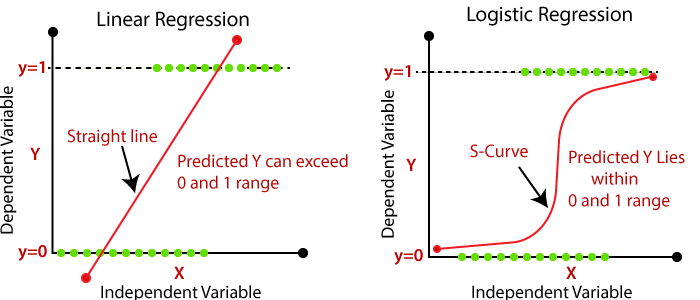
\includegraphics[scale=0.3]{images/image4.png}  
      \end{figure}


\textbf{Algoritmos Clasificación}
\begin{itemize}
    \item Árboles de desición
\end{itemize}

Los árboles de decisión es un método de clasificación que se asemeja a un árbol, en donde en la parte superior, la punta del árbol, también llamada nodo raíz se divide en ramas y hojas. Las ramas se dividen en más ramas o hojas, es decir que el árbol se hace más grande. Mientras que las hojas ya no cuentan con otra división disponible, el árbol ha terminado y se ha clasificado algo. El objetivo principal de los árboles es llegar a un punto en donde ya no se divida en más ramas y llegar a una hoja clasificatoria. Una vez que se llega ahí el algoritmo ha terminado. 

Un término importante para comprender cómo iniciar el árbol y que servirá como raíz de la misma es utilizando la impureza de sus hojas, la pregunta que ayude a determinar si existe una enfermedad y que tenga la menor impureza servirá para ser la siguiente rama. La impureza de una hoja  se refiere a la mezcla o variedad de las clases en la misma. Es decir, en una hoja del árbol, la impureza mide cuánto las instancias de diferentes clases están mezcladas. Cuanto menor sea la impureza de la hoja, más pura será, lo que significa que contiene principalmente instancias de una sola clase. La impureza se utiliza en la selección de la mejor división en un árbol de decisión, ya que el objetivo es minimizar la impureza de las hojas. Hay varios métodos para medir la impureza de una hoja; este escrito utilizará la impureza de gini la cual  mide la probabilidad de clasificar erróneamente una instancia de forma aleatoria. Cuanto mayor sea la probabilidad, mayor será la impureza de la hoja. Lo deseado es tener la menor impureza posible cuanto antes para lograr hacer los algoritmos de clasificación veloz.  Un árbol de decisión se verá como la figura 3 a continuación. 
Para esta aplicación dado que se está prediciendo categorías, el árbol generado será un árbol de clasificación. \cite{SQ4}



\begin{figure}[h!]
  \caption{\csentence{}
      Ejemplo árboles de desición}
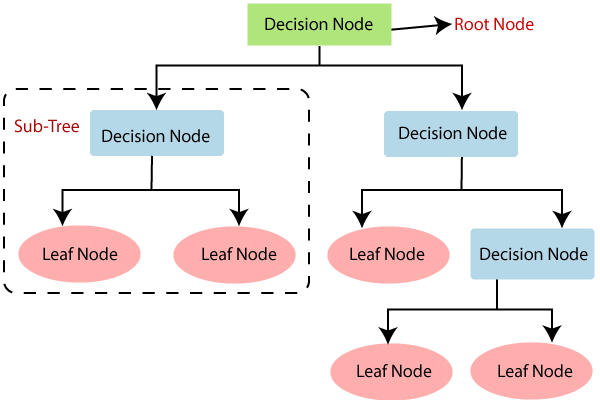
\includegraphics[scale=0.21]{images/DT.png}  
      \end{figure}

Se ha particionado los datos en un conjunto de entrenamiento y otro prueba para poder evaluar el desempeño de los modelos de arbol de desición y regresión logística.Para ello es importante definir cómo se calculan los métricos de desempeño y cómo se interpretan: 

\begin{itemize}
 \item Regresión Logística
        \subitem Matriz Confusión: Matriz dos por dos que muestra la cantidad de los cuatro escenarios posibles de predicción. Verdaderos positivos, verdaderos falsos, falsos positivos y falsos negativos.
\begin{figure}[h!]
  \caption{\csentence{}
      Matriz de confusión}
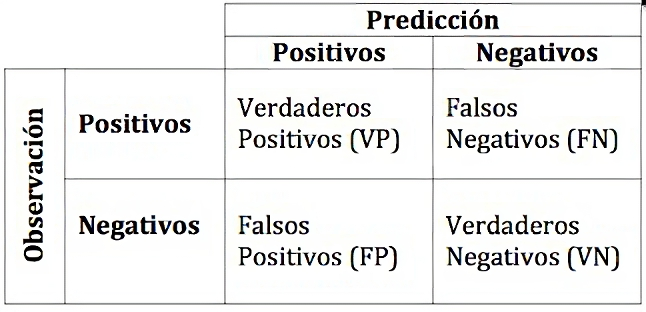
\includegraphics[scale=.3]{images/Mc.png}  
      \end{figure}
        
        \subitem Curva ROC: \textit{Reciever operation characteristic} por sus siglas en inglés muestra la relación entre la tasa de verdaderos positivos (tasa de detección) y la tasa de falsos positivos (tasa de error) para diferentes umbrales de decisión del modelo.El punto (0,0) en el gráfico representa la tasa de falsos positivos y la tasa de verdaderos positivos cuando se clasifica todo como negativo. El punto (1,1) representa la tasa de verdaderos positivos y la tasa de falsos positivos cuando se clasifica todo como positivo.Una curva ROC ideal se acerca al punto (0,1), lo que indica una tasa de detección perfecta y una tasa de error mínima.La línea diagonal del gráfico representa un modelo con un rendimiento aleatorio.El área bajo la curva (AUC) es una medida de la precisión del modelo, donde un AUC de 1.0 indica un modelo perfecto y un AUC de 0.5 indica un modelo que no tiene mejor rendimiento que un modelo aleatorio.La figura 5 muestra los diferentes escearios para gráficamente evaluar el desempeño de un algoritmo. \cite{SQ5}
        
\begin{figure}[h!]
  \caption{\csentence{}
      Curva ROC en diferentes escenarios}
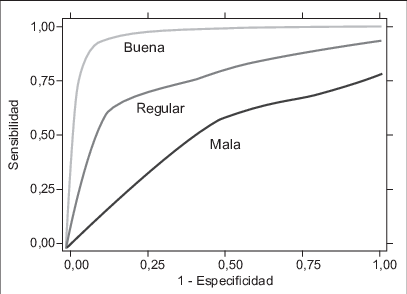
\includegraphics[scale=.8]{images/ROC.png}  
      \end{figure}
        
    \item Árboles de desición
        \subitem Accuracy:Proporción de clasificaciónes positivas que fueron correctas 
            \begin{equation}
            (V P+V N) /(V P+V N+F P+F N)
            \end{equation}


        \subitem Precision: proporción de clasificaciones verdaderas positivas entre las clasificaciones verdaderas

            \begin{equation}
            V P /(V P+F P)
            \end{equation}
        \subitem Recall: proporción de verdaderos positivos dados todos los positivos.
            \begin{equation}
                        V N /(V N+F P)
            \end{equation}


\section*{Resultados y discusión}

\textbf{Selección de características}

Como se mencionó en la metodología para entender cuáles son las variables que más podrían estar aportando al modelo se realizaron dos procedimientos, selección de características basadas en correlación y  selección de características basada en información mutua. Sabiendo que se cuentan con 142 variables y que realizar su matriz de rigidez sería complicada de visualizar, con ayuda de la exploración de datos realizada en la introducción se sabe que 10 síntomas son los que más incidencia deben de tener sobre la respuesta de presencia de diabetes.La figura 6 muesta las correlaciónes de cada variable con la presencia de diabetes. Las correlaciónes tienen los siguientes valores. 

$$
\begin{array}{cc}
\text { increased appetite } & 1 \\
\text { polyuria } & 1 \\
\text { weight_loss } & 0.47 \\
\text { irregular sugar level } & 0.97 \\
\text { blurred and distorted vision } & 0.55 \\
\text { fatigue } & 0.18 \\
\text { lethargy } & 0.47 \\
\text { restlessness } & 0.68 \\
\text { excessive hunger } & 0.46 \\
\text { obesity } & 0.68
\end{array}
$$

Con los resultados anteriores, se destaca que las variables que podrían tener mayor relevancia son el apetito incrementadto, la poliuria, valores irregulares de azúcar y obesisdad. Esta era una de las teorías propuestas en la introducción y se ha confirmado. Estas cuatro variables son candidatas a siempre ser requeridas tener información sobre el paciente para determinar si cuenta con diabetes. La ausencia de información de una de ellas podría hacer que la predicción no sea buena. Sin embargo hay que considerar que esta metodología únicamente considera las relaciónes lineales entre la variables de respuesta a la de salida y no está considerando la interacción entre ellas mismas. 

Paro poder lograr lo anterior también se realizó una prueba de selección de caracteristicas de inforamción mutua para compreneder la interacción entre las variables predictoras. A continuación sus resultados para las 5 interacciónes más fuertes. La información mutua es una medida de la cantidad de información que dos variables comparten. En el contexto de la selección de características, la información mutua se puede utilizar para cuantificar la cantidad de información que una característica proporciona sobre la variable objetivo.
Más específicamente, la información mutua mide la reducción en la incertidumbre sobre la variable objetivo que se logra al conocer el valor de una característica. Cuanto mayor sea el puntaje de información mutua entre una característica y la variable objetivo, más información proporciona esa característica sobre el objetivo, y es más probable que sea útil para predecir la variable objetivo. En este caso se confirma de nueva cuenta que la polyuria, apetito incrementado, y mediciónes irregulares de azúcar son las más relevantes para predecir la respuesta. 

$$
\begin{array}{ll}
\text { polyuria } & 0.11 \\
\text { increased_appetite } & 0.11 \\
\text { irregular_sugar_level } & 0.10 \\
\text { restlessness } & 0.07 \\
\text { obesity } & 0.07
\end{array}
$$

\begin{figure}[h!]
  \caption{\csentence{}
     Matriz de correlación de las 10 variables más importantes para presencia de Diabetes y la respuesta de diabtes. }
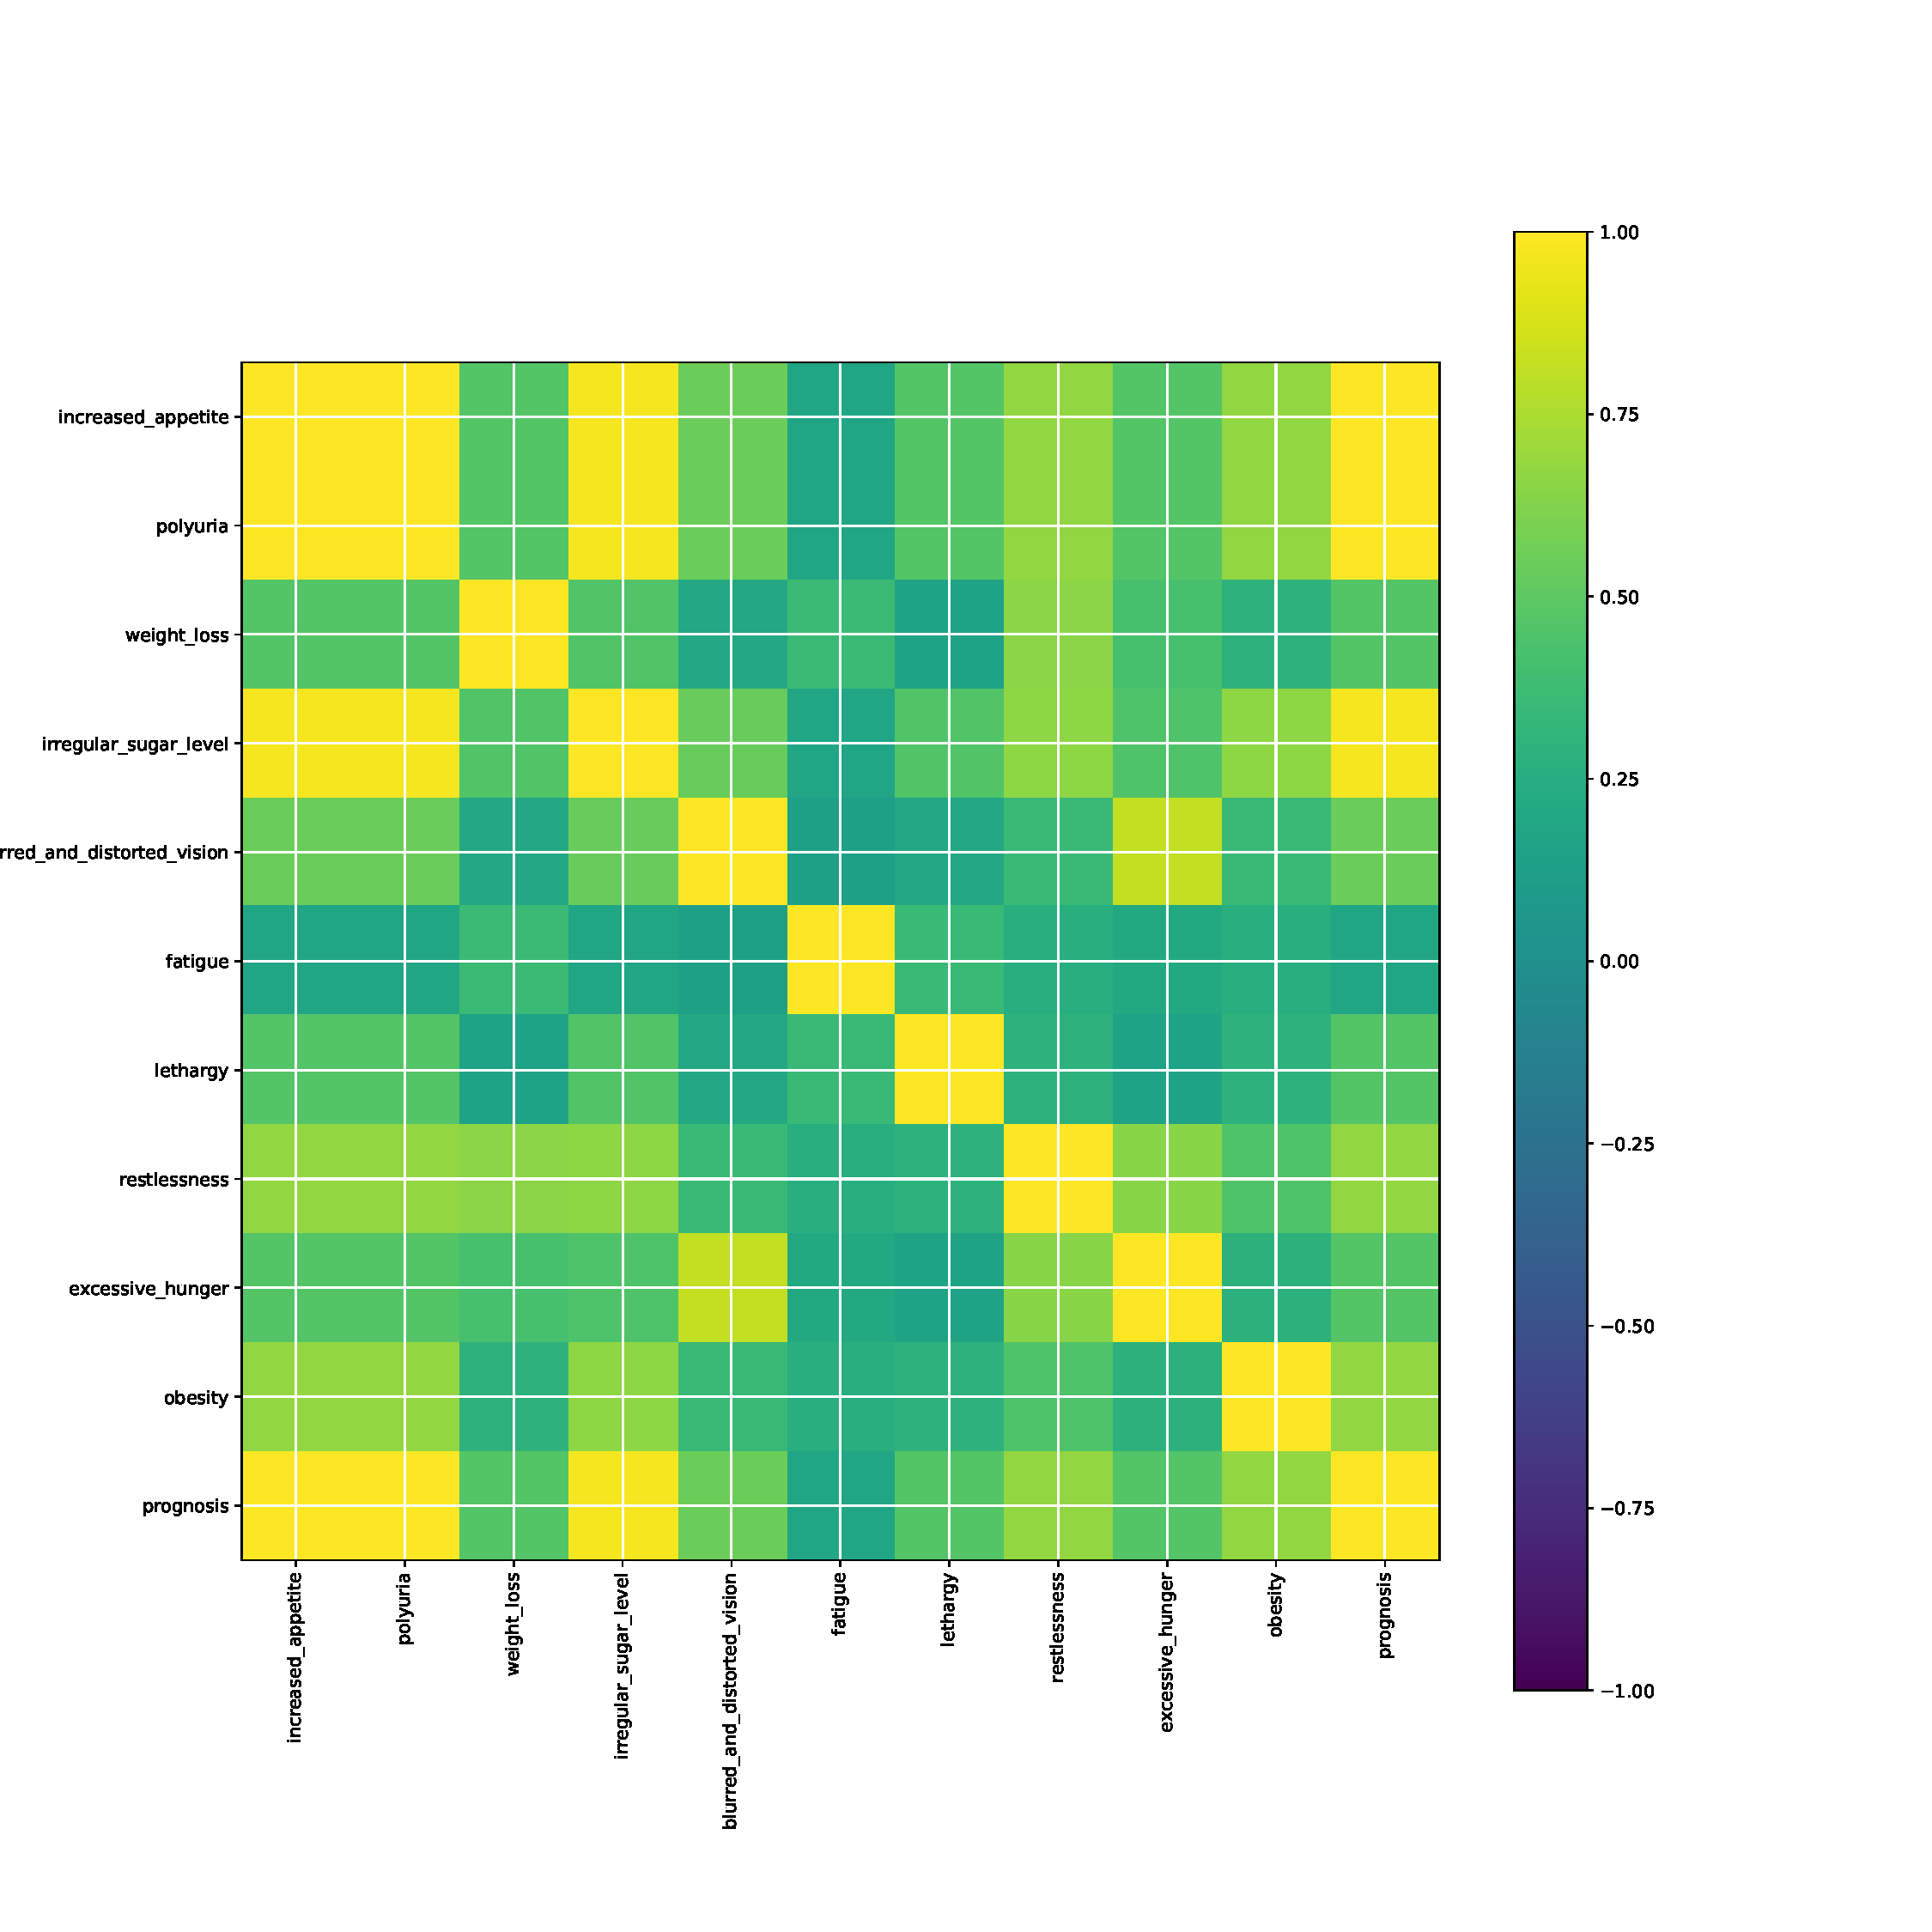
\includegraphics[scale=.2]{images/correl.pdf}  
      \end{figure}


\textbf{Aprendizaje No supervisado}

Como se explicó en la introducción, se llegó a la conclusión que aprendizaje no supervisado por medio de K medias o DBSCAN no era adecuado para evaluar información binaria dado que esta ya cuenta con una etiqueta de clasificación implícita, la presencia o no de una enfermedad o síntoma. Esto es solo una conclusión personal y se desea explorar más las veracidad de dicha aseveración. Para ello y como trabajo futuro se tendrá una plática con el profesor para comprender que podría estar siendo interpretado incorrectamente para poder complementar esta sección. 

De todas maneras con el objetivo de aprendizaje académico el algoritmo se corrió para obtener el siguiente gráfico de dispersión de la siguiente figura comparando las dos variables de mayor relevancia encontras en la selección de características. Es muy evidente que solo se cuentan con dos grupos, lo cual es lógico, siendo ausencia o presencia de la enfermedad. En realidad debieron haber sido 4 grupos (que se tenga ambos síntomas, que tenga uno pero no el otro y viceversa y que tenga ambos), sin embargo para los 120 pacientes diagnosticados con diabetes, todos cuentan con ambos síntomas. En esta sección no se presentan los resultados de DBSCAN por que las conclusiones son similares. Sería necesario proponer otro algoritmo de aprendizaje no supervisado para encontrar patrones no encontrados visualmente dado que se cuenta con 142 grados de libertad.


\begin{figure}[h!]
  \caption{\csentence{}
      Grafico dispersión K meadias con dos centroides}
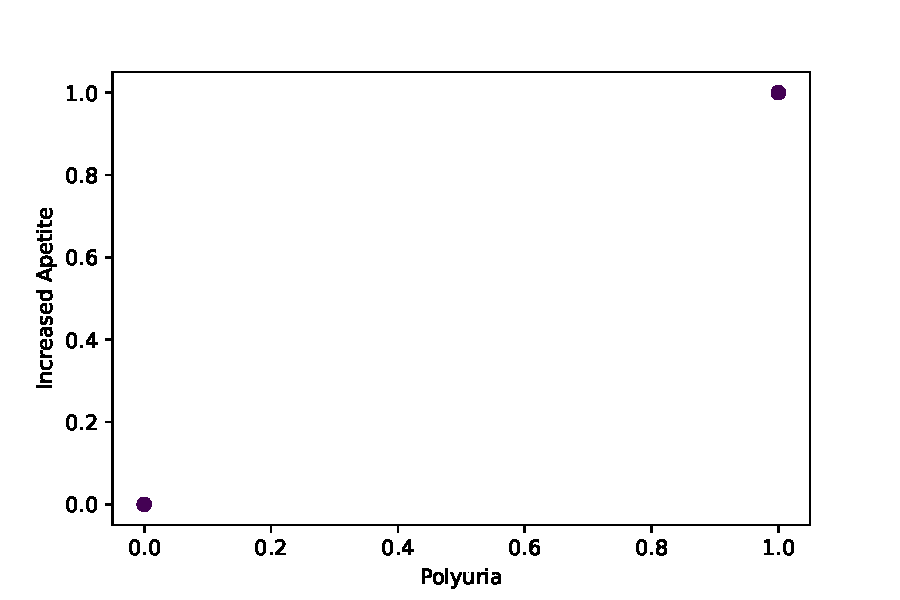
\includegraphics[scale=.45]{images/kmeans.pdf}  
      \end{figure}
        
\textbf{Aprendizaje supervisado}

Regresión Logística

Para poder realizar la regresión logística se partió el conjunto total de pacientes en 70 porciento entrenamiento y 30 porciento pruebas. Esto genera un total de 3,445 pacientes para entrenamiento y 1,475 pacientes para pruebas. 

Siguiendo los pasos descritos en la metodología para el conjunto de entrenamiento , y utilizando la precisión como métrico se obtiene que su resultado es de 1. Lo cual quiere decir que los datos nuevos el algoritmo pudo predecir correctamente todos las clasificaciones positivas. Esto quiere decir que para los 1,475 pacientes acertó para todos en determinar si el paciente tiene diabetes o no. 
$$
\text { Presición : } 1.0
$$
La figura 8 muestra la matriz de confusión donde se demuestra que se predijeron correctamente 36 casos de diabetes y 1,439 pacientes fueron clasifcados correctamente en no tener diabetes. 

\begin{figure}[h!]
  \caption{\csentence{}
      Grafico dispersión K meadias con dos centroides}
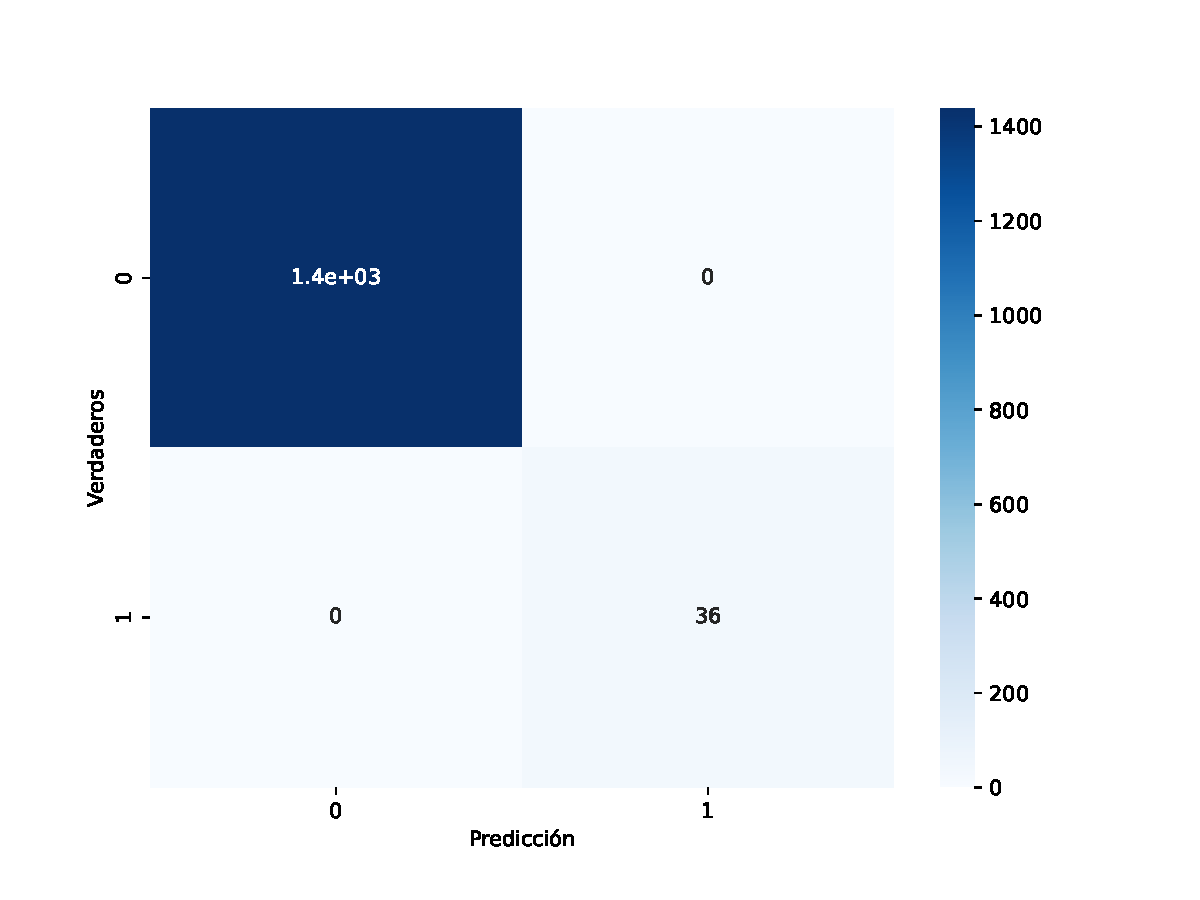
\includegraphics[scale=.45]{images/matrizconf.pdf}  
      \end{figure}

Finalmente la figura 9 muestra la curva ROC, en donde se demuestra un comportamiento de predicción perfecto, lo cual hace sentido con la matriz de confusión, es por eso que la curva no es una curva si no una linea horizontal perfecta en el eje x con valor de 1. Esto quiere decir que el algoritmo funciona a la perfección. 

\begin{figure}[h!]
  \caption{\csentence{}
      Grafico ROC para evaluar desempeño de regresión logística}
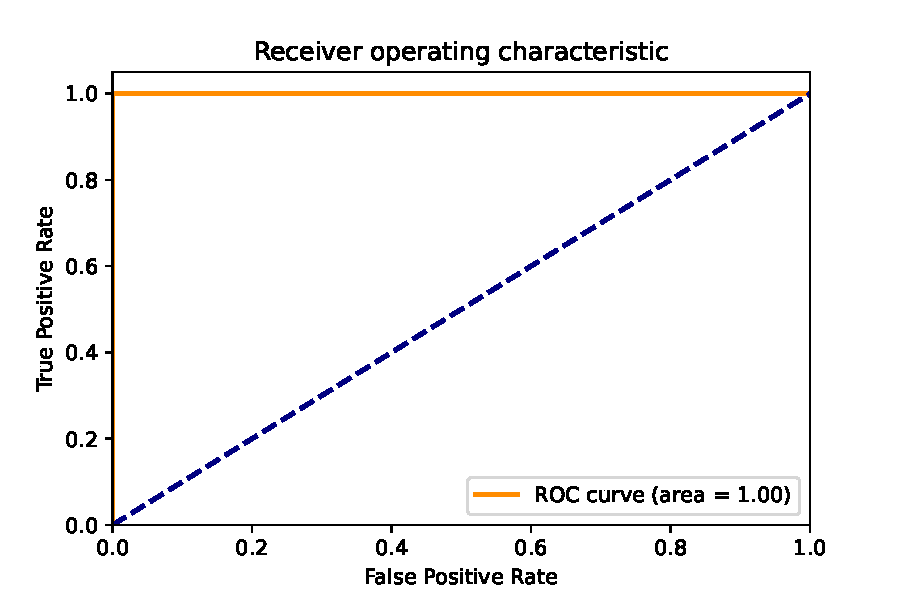
\includegraphics[scale=.45]{images/ROCC.pdf}  
      \end{figure}



\textbf{Clasificación}

Para la clasificación se utilizó un algoritmo de árboles de decisión para encontrar el camino más eficiente para clasificar a un paciente con diabetes. Siguiendo el algoritmo descrito en metodología el árbol como la figura 10. Lo que quiere decir este árbol es que según la incidencia de la 104 la cual corresponde la presencia de poliuria,  para este conjunto de datos en específico es suficiente para determinar si el paciente tiene diabetes o no. Con solo cuestionar al paciente si está presente puede ayudar mucho a entender la diabetes, Esto tiene sentido dado que en secciones anteriores se había encontrado que absolutamente todos los pacientes que reportaban tener poliuria tenían diabetes es decir, no hay ninguna otra enfermedad que tenga este síntoma. Solo se cuenta con una raíz y dos hojas. En este caso la impureza de gini es de 0, lo deseado, dado que esta variable solo aparece en diabetes. Para este caso se determina que solamente 84 pacientes del conjunto de entrenamiento cuenta con diabetes por lo que 36 del set de prueba también lo tendrán.misma conclusión encontrada en el algoritmo de  regresión logística. 

\begin{figure}[h!]
  \caption{\csentence{}
      Árbol de desicion para poliuria}
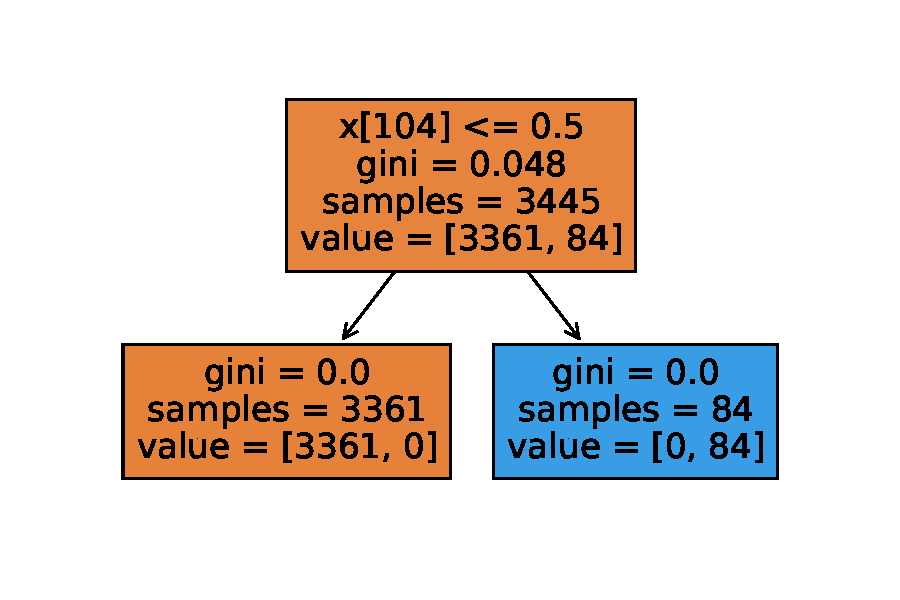
\includegraphics[scale=.45]{images/DT1.pdf}  
      \end{figure}


Es interesante cuestionarse qué sucedería si no se tuviera información respecto a la polyuria, cómo quedaría el diagrama de árbol. Para dar respuesta a ello se elimina la polyuria y ahora la variable dominantes el apetito incrementado el cual también genera un árbol de un solo nivel dado que este síntoma únicamente está presente en la diabetes. Hacer este árbol lleva a la misma cantidad de pacientes clasificados con diabetes. 

\begin{figure}[h!]
  \caption{\csentence{}
      Árbol de desicion para apetito incrementado}
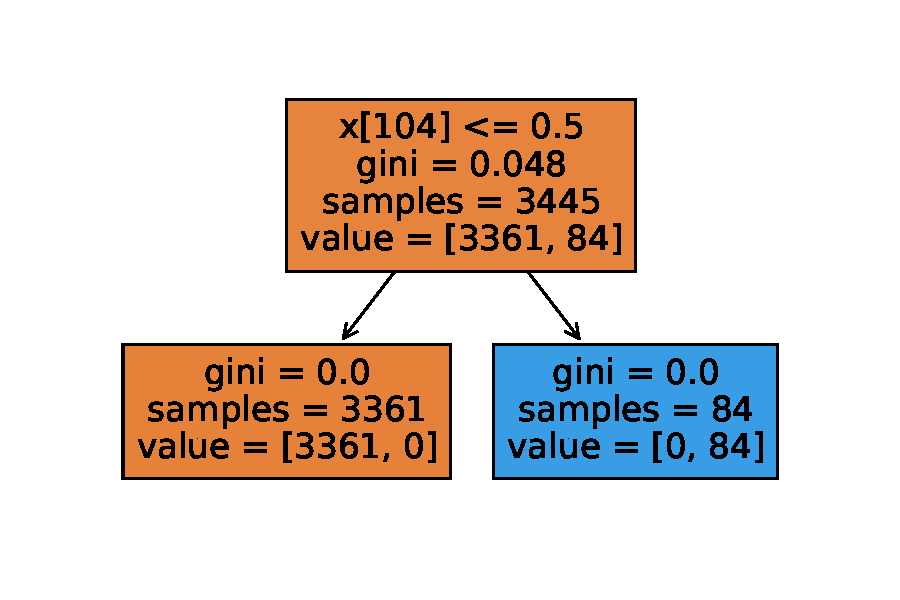
\includegraphics[scale=.45]{images/DT2.pdf}  
      \end{figure}

Ambos algoritmos obtienen las siguientes métricos de desempeño: 

Accuracy: 1.0
Precision: 1.0
Recal1: 1.0
F1-score: 1.0


\section*{Conclusión}

De los algoritmos de aprendizaje automático se concluye que:  
\item Para el conjunto de datos estudiado, si es posible dictaminar con un excelente desempeño si un paciente padece diabetes o no. Los algoritmos de regresión logística, árboles de decisión y bayes ingenuos muestran excelencia al clasificar la presencia o ausencia de diabetes ya que los tres clasifican correctamente a todos los pacientes del conjunto de prueba. La información brindada por los síntomas es suficiente para hacer predicción de conclusiones médicas. 
\begin{itemize}
    \item Esto se comprueba con los métricos de desempeño como la precisión, exactitud, y F1 los cuáles todos tienen un valor de 1. De la misma manera las curvas ROC muestran una línea horizontal perfecta en y = 1 
\end{itemize}

\item Si bien esto es lo deseado, se sospechó que algo pudiera estar mal en el conjunto de datos. Investigando en el foro donde se obtuvo la información se encontró que solo se cuentan con 304 registros únicos dentro de los 4,920 pacientes, se tienen muchos pacientes repetidos (con exactamente la misma combinación de síntomas). Esto lo que genera sobreajuste haciendo que los modelos funcionen de manera excelente como muestra el punto anterior, pero únicamente con este conjunto de datos. Esto deja la lección aprendida de revisar la calidad de los datos antes de comenzar a trabajarlos, en este caso entender si existen pacientes repetidos.  


\item Los algoritmos dejan entrever que los síntomas que son más relevantes para comprender si un paciente pudiera tener diabetes es la polyuria, el apetito incrementado y niveles irregulares de azúcar en la sangre. La ausencia de saber información de estos síntomas pudiera comprometer a los algoritmos para entender si se diagnostica diabetes. 

\item Comparar cuál algoritmo tiene un mejor desempeño que otro, para este caso en particular carece de sentido dado que todos obtuvieron desempeños perfectos. 

\item Como trabajo futuro se desea compilar las lecciones aprendidas del presente sobre otro conjunto de datos que cuenta con mayor calidad en sus datos para llegar a conclusiones de un valor agregado mayor a las actuales que funcionan principalmente con fines educativos. 










%%%%%%%%%%%%%%%%%%%%%%%%%%%%%%%%%%%%%%%%%%%%%%
%%                                          %%
%% Backmatter begins here                   %%
%%                                          %%
%%%%%%%%%%%%%%%%%%%%%%%%%%%%%%%%%%%%%%%%%%%%%%

\begin{backmatter}

%%%%%%%%%%%%%%%%%%%%%%%%%%%%%%%%%%%%%%%%%%%%%%%%%%%%%%%%%%%%%
%%                  The Bibliography                       %%
%%                                                         %%
%%  Bmc_mathpys.bst  will be used to                       %%
%%  create a .BBL file for submission.                     %%
%%  After submission of the .TEX file,                     %%
%%  you will be prompted to submit your .BBL file.         %%
%%                                                         %%
%%                                                         %%
%%  Note that the displayed Bibliography will not          %%
%%  necessarily be rendered by Latex exactly as specified  %%
%%  in the online Instructions for Authors.                %%
%%                                                         %%
%%%%%%%%%%%%%%%%%%%%%%%%%%%%%%%%%%%%%%%%%%%%%%%%%%%%%%%%%%%%%

% if your bibliography is in bibtex format, use those commands:
\bibliographystyle{bmc-mathphys} % Style BST file (bmc-mathphys, vancouver, spbasic).
\bibliography{bmc_article}      % Bibliography file (usually '*.bib' )
% for author-year bibliography (bmc-mathphys or spbasic)
% a) write to bib file (bmc-mathphys only)
 %@settings{label, options="nameyear"}
% b) uncomment next line
%\nocite{label}

% or include bibliography directly:
%\begin{thebibliography}

%&\end{thebibliography}

%%%%%%%%%%%%%%%%%%%%%%%%%%%%%%%%%%%
%%                               %%
%% Figures                       %%
%%                               %%
%% NB: this is for captions and  %%
%% Titles. All graphics must be  %%
%% submitted separately and NOT  %%
%% included in the Tex document  %%
%%                               %%
%%%%%%%%%%%%%%%%%%%%%%%%%%%%%%%%%%%

%%
%% Do not use \listoffigures as most will included as separate files


\end{backmatter}
\end{document}
